\hspace{1.5cm}
Segundo o ENVI\cite{envi}, este sistema é usado para construção de um novo arquivo com imagens georeferenciada. As bandas são reamostradas e re-projetada em projeções e tamanho de pixel compativeis. Todas as imagens são compactadas em um unico arquivo, o facilita a manipulação das mesma. 

\begin{itemize}
\item \textbf{Basic Tools}
\begin{itemize}
\item\textbf{ Layer Stacking}\\

\end{itemize}
\begin{figure}[!htpb]
        \centering
        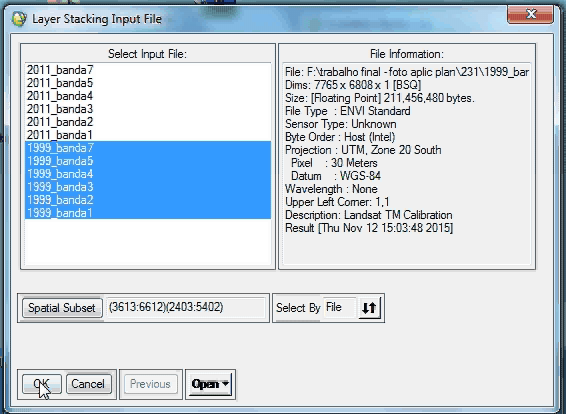
\includegraphics[scale=0.4]{imagens/empilhamento01.png}
        \caption{Escolha dos arquivos para empilhamento.}
        \label{empilhamento01}
\end{figure}        
\begin{figure}[!htpb]        
        \centering
        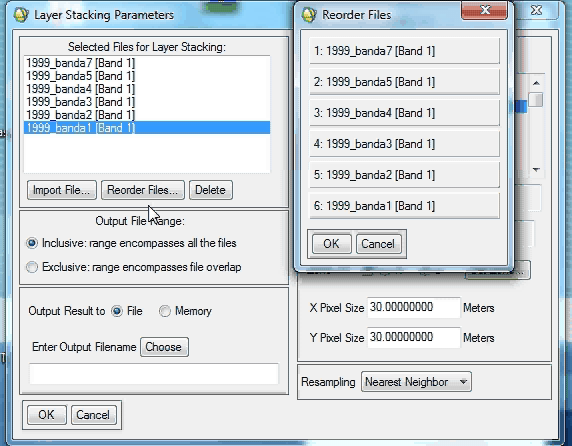
\includegraphics[scale=0.4]{imagens/empilhamento03.png}
        \caption{Reordenação das Bandas.}
        \label{empilhamento03}
\end{figure}        
\begin{figure}[!htpb]        
        \centering
        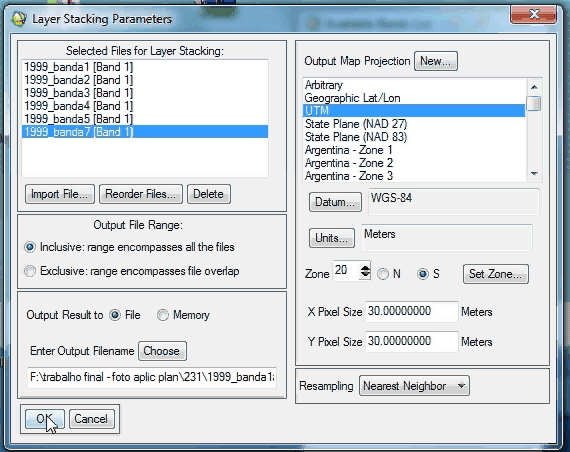
\includegraphics[scale=0.4]{imagens/empilhamento05.png}
        \caption{Nome do arquivo com as Bandas.}
        \label{empilhamento05}
\end{figure}
\end{itemize}
\hspace{1.5cm}
Depois de corte das imagens na tela de parâmetros com as bandas já selecionadas, clica no botão \textbf{Import File}, conforme figura \ref{empilhamento01}.Na próxima janela é necessário a reordenação das imagens, através do botão \textbf{Reorder Files}, figura \ref{empilhamento03}. Depois escolher o local/nome do arquivo e realizar a criação do empilhamento das bandas, figura \ref{empilhamento05}. 
